\label{chapter:hla3}
In this chapter, we introduce different clustering technique in Section \ref{hla3:approach}. Next, we present a  human-subject study of the developed HCPC tool in Section \ref{hla3:human_study}. In Section \ref{hla3:interface} and \ref{hla3:implementation}, we discuss the interface and implementation of the HCPC tool. Last, in Section \ref{hla3:use_guide} and \ref{hla3:case_study}, we discuss how to use HCPC tool for two use cases and present an example using \emph{jupyter\_client} project.

\section{Motivation}
Finding relevant methods, classes and files are frequent part of daily activities of a software developer. Most of the software maintenance tasks require to find relevant locations for solving the task. As the size of codebase grows, it becomes difficult to remember everything in detail. Therefore, common practice is to figure out some relevant keywords and search for the files containing the keywords. The problem with this approach is search results are random and it gives no idea of exploring the codebase according to the order different components are called.

In the previous studies, we have advanced the existing works on hierarchical abstraction of static execution paths by finding appropriate techniques to label nodes in the tree and further complement the nodes with natural text summary and execution patterns for better comprehension. In this study, our motivation is to make the abstraction tree usable for developers' daily concept location activities. We have found two areas for improvement on the previous studies. First, we observe the abstraction tree became complex to explore as the number of execution paths grows. Therefore, we implemented a cluster flattening technique to have more flexibility and simple structure with cut-off depth. Second, we have changed the similarity metric for comparing execution paths from Jaccard distance to match\_a\_strike score. By updating the similarity measure, we ensure more accurate grouping of clusters. After the technique changes, we have developed a tool called HCPC for doing a human-subject study to find the effectiveness of HCPC. In the HCPC tool, we added a node highlight feature where specific function can be selected to highlight relevant nodes. From our study with developers, we have found that the HCPC tool can be helpful for exploring the codebase in a guided way in daily software maintenance activities. 



\section{Approach}
\label{hla3:approach}
In this study, we have followed similar steps as study 1 and 2 except two changes. First, we have changed the similarity score from Jaccard distance to strike\_a\_match algorithm. The strike\_a\_match algorithm takes into account the contents of two lists and the sequence they appear. On the contrary, Jaccard distance only considers the content of two lists. To improve the clustering result, we have made the change in similarity metrics. Second, we have added one more step to reach the final abstract code summary tree. Previously we have used the step by step tree returned by a linkage algorithm. However, the linkage tree is not flexible for browsing. Therefore, we have used a cluster flattening technique to get more flexible 5-6 depth tree. We discuss strike\_a\_match, node summary, execution pattern and cluster flattening techniques in the following subsections. 

\subsection{strike\_a\_match}
In Algorithm \ref{alg:strike_a_match}, we provided the pseudo code for reproducing the strike\_a\_match algorithm\footnote{http://www.catalysoft.com/articles/strikeamatch.html}. The method takes input two lists which are execution paths one and two. The method returns a similarity score between 0 and 1 where 0 means no match and 1 means full match. In line 2-3, all method pairs in consecutive order are generated. In line 4, we calculate union value by summing length of the two generated pair lists. From line 6 to 14, we iterate over the pair lists and see if they match to calculate intersection value. When we find a match, we remove the pair from $ep2\_pairs$ to avoid considering the same match again. Finally, we return the similarity score using union and intersection values. The method considers the order in addition to the content of two lists. 


\begin{algorithm}
    \SetKwInOut{Input}{Input}
    \SetKwInOut{Output}{Output}
    
    \underline{Compare\_execution\_paths} 
    
    \Input{ep1, ep2}
    \Output{similarity\_score}
    \tcp{method\_pairs returns all the two length consecutive pairs from execution paths}
    ep1\_pairs = method\_pairs(ep1)\; 
    ep2\_pairs = method\_pairs(ep2)\;
    union = len(ep1\_pairs) + len(ep2\_pairs)\;
    intersection = 0\;
    
    \For{$i\gets0$ \KwTo $len(ep1\_pairs)$ }{
        \For{$j\gets0$ \KwTo $len(ep2\_pairs)$ }{
            
            \If{ep1\_pairs[i] == ep2\_pairs[j]}{
                intersection += 1 \;
                ep2\_pairs.pop(j)\;
                \textbf{break}\;
            }
        }
    }
    \textbf{return} ( 2 * intersection) / union
    
    \caption{Strike\_A\_Match algorithm}
    \label{alg:strike_a_match}
\end{algorithm}

\subsection{Node Summary}

In Algorithm \ref{alg:node_summary}, we provided the pseudo code for generating a node summary for each abstraction node. The two input of the method are execution paths and function\_id to comment dictionary. The execution paths are in a 2D list where each row corresponds to an execution path and the cells contain function id. The second argument is a dictionary where function id are mapped to their first line docstring comment. In line 3 - 7, we iterate through all the execution paths and all functions in an execution path. We add all the comments to $all\_comments$ variable for use in summarize. In line 8, we provoke the summarize method from Gensim~\cite{gensim} library which by default returns one-third of the $all\_comments$ as summary using the TextRank~\cite{mihalcea2004textrank} algorithm. We have tried with different ratios of input to summary and found the default settings sufficient for our purpose.

\begin{algorithm}
    \SetKwInOut{Input}{Input}
    \SetKwInOut{Output}{Output}

    \underline{Generate\_node\_summary} 
    
    \Input{execution\_paths, function\_id\_to\_comment}
    \Output{node\_summary}
    all\_comments = ` '\;
    \For{execution\_path \textbf{in} execution\_paths}
    {
        \For{function\_id \textbf{in} execution\_path}
        {
            all\_comments += function\_id\_to\_comment[function\_id]\;
        }
    }
    
    node\_summary = summarize(all\_comments)\; \tcp{summarize by Gensim}
    \textbf{return} node\_summary
    \caption{Generate node summary from execution paths of an abstraction node}
    \label{alg:node_summary}
\end{algorithm}

\subsection{Execution Patterns}
In Algorithm \ref{alg:execution_patterns}, we present pseudo code for generating execution patterns. The method takes execution paths as input and outputs frequent patterns found by analyzing all the execution paths. For our approach, we have mined the top-15 most frequent patterns. Execution paths is a list of lists of function ids which can be called sequentially. We use the PrefixSpan algorithm which mines frequent patterns from a set of lists. We use the topk method to get the top-15 execution patterns. We use default settings for maximum length and minimum length of the patterns. 

\begin{algorithm}
    \SetKwInOut{Input}{Input}
    \SetKwInOut{Output}{Output}
    
    \underline{Generate\_Execution\_Patterns} 
    
    \Input{execution\_paths}
    \Output{execution\_patterns}
    NUMBER\_OF\_PATTERNS = 15\;
    ps = PrefixSpan(execution\_paths)\;
    top\_patterns = ps.topk(NUMBER\_OF\_PATTERNS)\; 
    
    \textbf{return} top\_patterns\;
    \caption{Generate node summary from execution paths of an abstraction node}
    \label{alg:execution_patterns}
\end{algorithm}


\subsection{Cluster Flatten Technique}

In previous studies, we have used a step-by-step clustering tree as the abstract code summary tree. However, for $n$ number of execution paths, the abstraction tree will have $2n + 1$ nodes which is not practical for medium to large projects. Therefore, we processed the cluster tree by using cluster flattening. The cluster flattening technique groups all clusters between a given distance as one. Therefore, by giving a larger distance, we can get very few clusters from a linkage matrix by merging all clusters between the distance as one. Similarly, we can get a larger number of clusters by using a small distance as the threshold value for flattening. For generating nodes at different depths, we use increasing threshold value for distance (e.g. [5, 4, 3, 2, 1.5]). We have manually tuned the distance values for individual subject systems.



\section{Implementation }
\label{hla3:implementation}
In this section, we briefly highlight different parts of our implementation as shown in Figure \ref{fig:architecture}.

\begin{enumerate}
    \item We clone the source code from GitHub in a temporary folder. The source code will be used in the next phase by the Python static code analyzer.
    \item We use Pyan~\cite{pyan} as static Python code analyzer. Pyan goes through all the \emph{*.py} files looking for which method calls which method. Pyan generates a text file  which encodes all the methods with numbers and then contains which method calls which method. We generate static call graph using NetworkX~\cite{networkx} with the caller-callee relationships generated by Pyan.
    
\begin{figure*}[h]
\centering
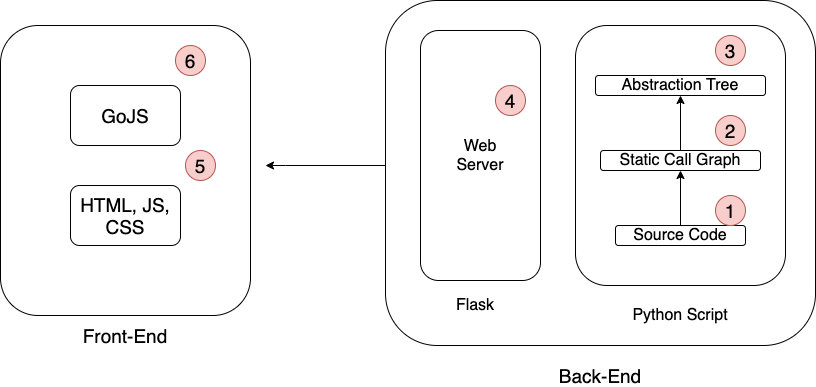
\includegraphics[width=\columnwidth]{figures/hla3/hla3_implementation.png}
\caption{Architecture of HCPC tool }~\label{fig:architecture}
\end{figure*}

    \item We generate execution paths from the call graph created in previous step.
Execution paths are grouped using the Agglomerative Hierarchical Clustering~(AHC) algorithm provided by the Scipy~\cite{scipy} library with \emph{ward} method as a  distance metric. We have a binary tree structure where leaf nodes are execution paths and other nodes are clusters at different levels. We call these cluster nodes abstraction nodes. The abstraction nodes have a collection of execution paths. For each abstraction node, we generate three properties. For each node, we create node title by applying information retrieval techniques ( Scikit-learn~\cite{scikit-learn} for TFIDF and Gensim~\cite{gensim} for LDA, LSI ) on the method names of all execution paths of a node. Then we produce node summary by summarizing (TextRank by Gensim) method comments of all the execution paths of the node. Last we generate execution patterns by pattern mining among the execution paths of the node~(PrefixSpan \cite{prefixspan}). We write all the node data in a text file. Data is written in JSON format where each node is keyed with their ID and they have parent\_id, node title, node summary, execution patterns and execution paths associated with them. 
    \item We have Flask server for interacting with front-end. Client requests which subject system they want to explore and the server returns JSON response with the abstraction tree. 
    \item For the interface of our web application, we have used HTML, CSS, and JQuery. When a specific node is right-clicked, detail information about the node is filled to the node details panel.
    \item We used GoJS for building the abstraction tree diagram. Each abstraction  is a GoJS node and different properties of the abstraction nodes are binded to GoJS nodes. 

\end{enumerate}


\section{Interface}
\label{hla3:interface}
In this section, we will discuss the different components of our HCPC tool shown in Figure \ref{fig:interface}.

\begin{itemize}
    \item \textbf{Abstract Tree Panel(A).} In the panel, the main abstraction tree is presented. The root nodes are presented vertically which can be possible to expand with their child nodes. By right clicking the mouse on a node will load different information of the abstraction node in the right side of the interface.
    \item \textbf{Number of execution paths(B).} As each node in the abstraction tree are a collection of execution paths, we show the number of execution paths for a selected node in this element.
    \item \textbf{Files (C).} In the element, we show the unique files of all the methods that the execution paths belong to.
    \item \textbf{Node summary (D).} In the element, we have provided natural text description of a node. When developers select a node, the text description of the node will appear in the element. 
    \item \textbf{Execution Patterns (E).} In the element, for a selected abstraction node, frequent function call patterns are presented with the file they are associated with. In the current setting, top-10 frequent execution patterns are shown. 
    
    \item \textbf{Execution paths (F).} In the element, we show five execution paths of a selected abstraction node. The execution paths complement the execution patterns by showing a glimpse of the real execution paths. Moreover, when a specific method is searched, the execution paths with the searched method is presented instead first five methods.
    
    \item \textbf{ Node label technique and search panel (G).} The panel has three drop-down boxes. First, developers can select which subject system they want to explore. Second, they can choose which technique to be used for labeling the nodes in abstraction tree. Third, this drop-down box is search enabled and it helps to highlight the nodes which have the searched method in their execution paths.
\end{itemize}

\begin{figure*}[h]
  \centering
  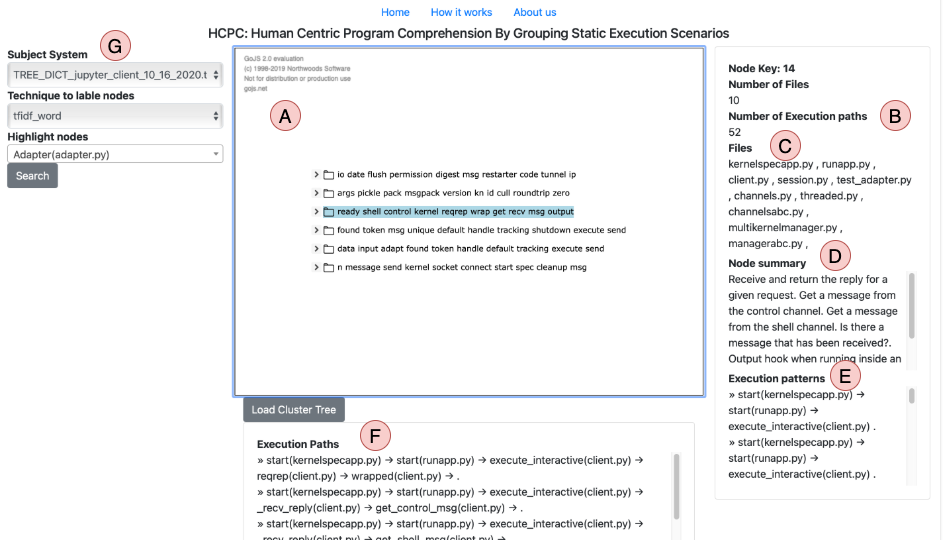
\includegraphics[width=\columnwidth]{figures/hla3/hla3_interface.png}
  \caption{HCPC tool interface }~\label{fig:interface}
\end{figure*}


\section{Guide to Use the HCPC Tool}
\label{hla3:use_guide}
The tool can be used in two ways. First, a developer new to the code-base can load the abstraction tree which starts with top abstraction  nodes. In the node details panel, for each node the number of execution paths, a brief natural text summary, and few frequent execution patterns are presented. Therefore, the developer can start first by observing summary and patterns of the top nodes. Now, the child nodes of the top nodes can be expanded and similarly explored by observing corresponding node summary and patterns. The developer can continue this way according to their need to get acquainted with the coda-base behavior and high-level concepts in the code-base.

Second, a new contributor to a open source project or someone new to a team can utilize the tool to understand high-level concepts related to a specific method. Developers first start from looking to open issues of a repository to find something work on. The issues are natural text description which provides information regarding a bug or a feature enhancement request. Developers can identify a few keywords and use our tool to find matching methods relevant to the keywords. Next, a specific method can be selected to highlight relevant nodes in the tree. The difference between the first approach here is developers will be able to browse the tree with focus to the selected method. The node titles relevant to selected methods will be highlighted so that the developer can expand their child nodes. In this way, the developer can navigate from the high-level concept to low-level source code related concepts for a specific method. By iterating this process, the developer can grasp high-level domain knowledge (with comment summary and IR techniques on function names) alongside insight into program execution scenarios which decreases the overhead due to lack of domain knowledge in the code-base. 

\section{Exploring HCPC for \emph{jupyter\_client} Project} 
\label{hla3:case_study}
\textbf{Exploring overview. } We have picked \emph{jupyter-client}\footnote{https://github.com/jupyter/jupyter\_client} as the subject system to show how the tool can be used following the two above mentioned techniques. To discuss the effectiveness of our tool using \emph{jupyter-client}, first we will discuss high level functionalities of \emph{jupyter-client} from their documentation. Later, we will present the information provided by our tool and discuss whether our tool provides similar or more information to comprehend the \emph{jupyter-client} project. \emph{jupyter-client} has three components. First, \emph{kernelspec} deals with specify different type of kernels from predefined files. Second, kernel manager which is responsible for start, stop and signaling kernels for different scenarios. Third, kernel client which is responsible for communicating with kernels for code execution and other tasks \footnote{https://jupyter-client.readthedocs.io/en/stable/index.html}. From the above components we can get an abstract idea of the features of \emph{jupyter-client}. Now, we will discuss the high-level features suggested by HCPC tool. Below we have listed few high-level node summary of the \emph{jupyter-client} project and discuss them with respect to the documentation.

\begin{figure*}[h]
  \centering
  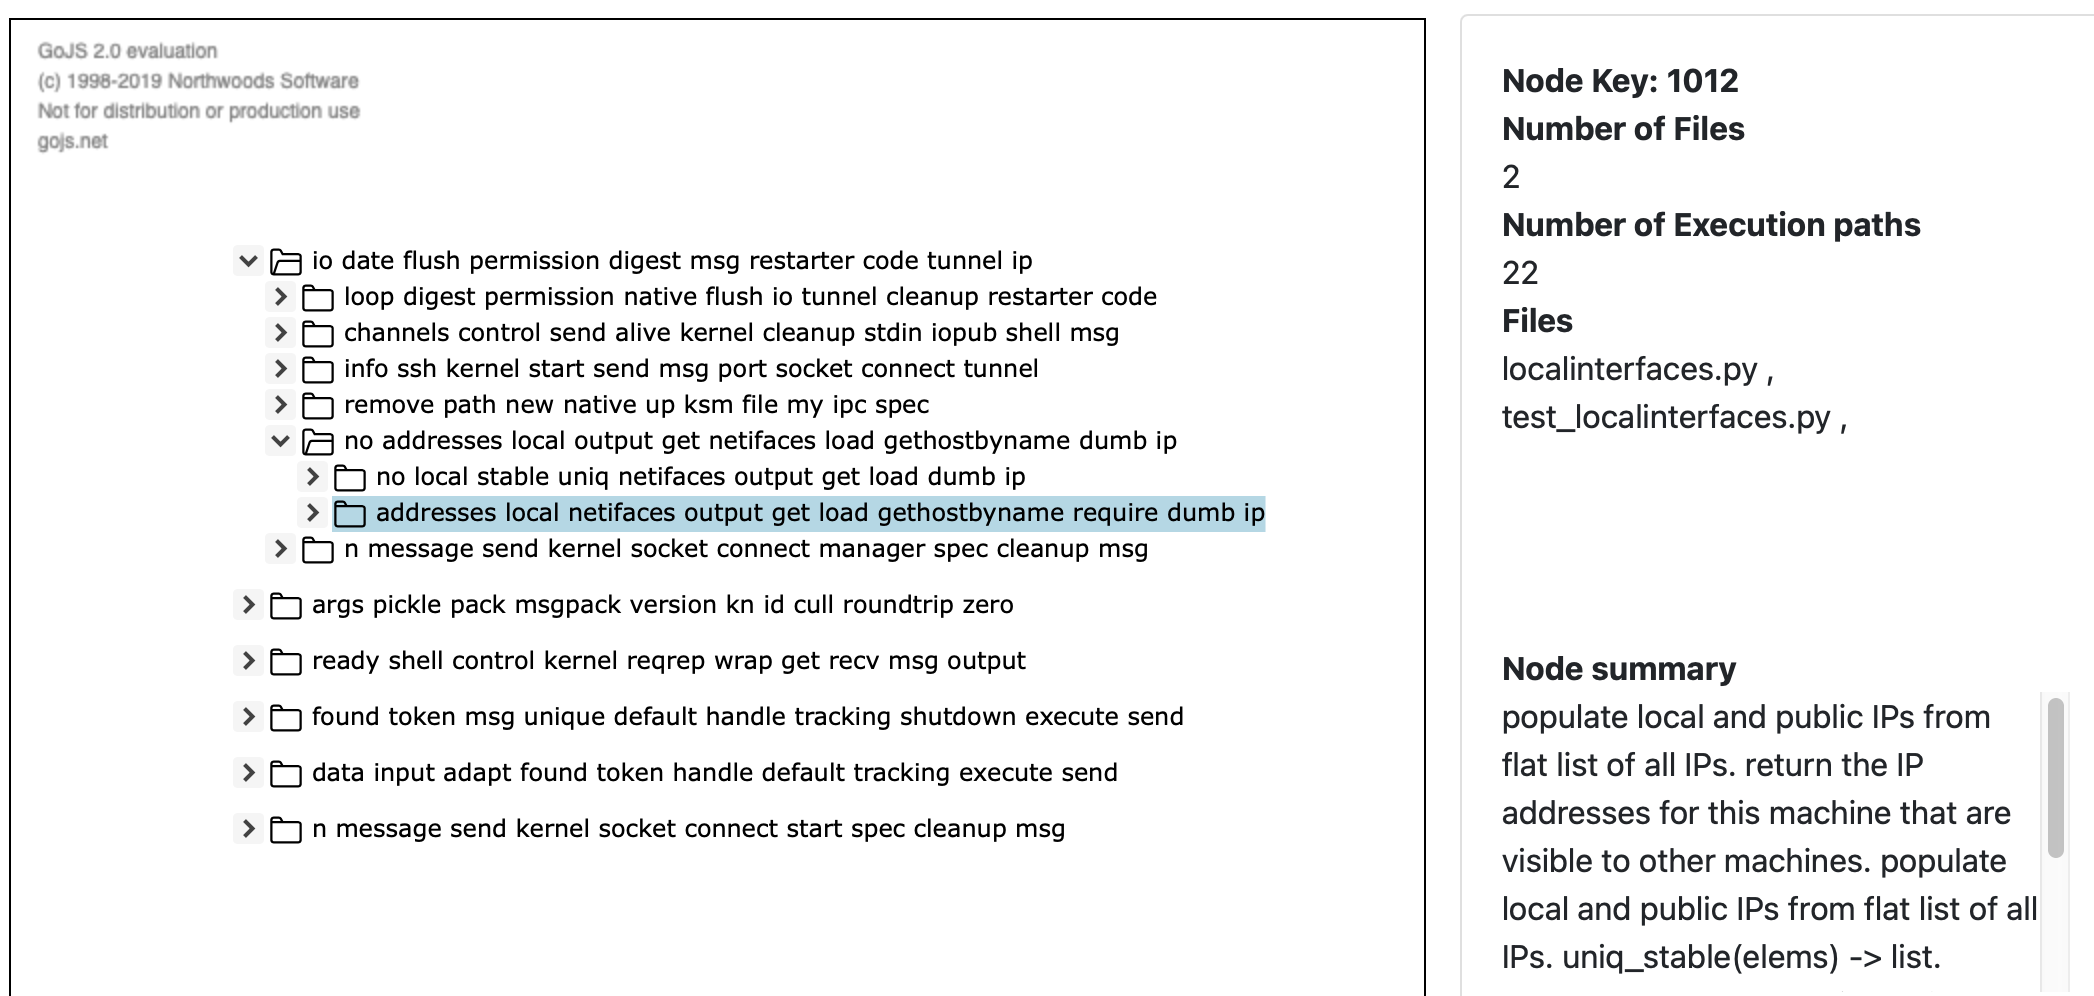
\includegraphics[width=\columnwidth]{figures/hla3/hla3_jupyter_overview.png}
  \caption{HCPC tool overview for jupyter\_client project }~\label{fig:tool_overview_jupyter_client}
\end{figure*}

\begin{itemize}
    \item \emph{ Restarts a kernel with the arguments that were used to launch it. Prepares a kernel for startup in a separate process. Write connection info to JSON dict in self.connection\_file. replace templated args (e.g. Verify realpath is used when formatting connection file). Walks env entries in templated\_env and applies possible substitutions from current env.} 
    
    From this node summary, we can understand \emph{jupyter\_client} restarting kernels, writing connection information to file and creates different kernel environments.
    
    \item \emph{Create a zmq Socket and connect it to the kernel. Start a new kernel, and return its Manager and Client. return zmq Socket connected to the Control channel. Get the stdin channel object for this kernel. Wait for kernel shutdown, then kill process if it doesn't shutdown. Pass a message to the ZMQ socket to send. return zmq Socket connected to the Heartbeat channel. Get the shell channel object for this kernel. Get the iopub channel object for this kernel. Get the control channel object for this kernel. Sends a signal to the process group of the kernel (this. Stops all the running channels for this kernel. return zmq Socket connected to the Shell channel. return zmq Socket connected to the IOPub channel. return zmq Socket connected to the StdIn channel.} 
    
    From this node summary, we observe that the \emph{jupyter\_client} project has ZMQ socket which helps with message communication. It has different channels like iopub, stdin, shell and Heartbeat channel.
    
    \item \emph{load the IPs that point to this machine. populate local and public IPs from flat list of all IPs. return the IP addresses that point to this machine.} 
    
    From this node summary, we can comprehend that the \emph{jupyter\_client} project also deals with public, local IP address of a machine. 

\end{itemize}

From the above text blocks, we can understand that \emph{jupyter-client} is relevant to working with kernels, it uses ZMQ socket to communicate with kernels, and deals with IP addresses of a machine. In addition to the above node summaries when developers see the execution patterns, they can very quickly learn about the domain knowledge of \emph{jupyter\_client} project.

\textbf{Exploring for specific task. } Next, it is possible to browse the tree by focusing on a specific method. In Figure \ref{fig:tool_write_connection_file}, we can see the nodes in the tree are marked to indicate they are relevant to write\_connection\_file method. Developers can investigate the nodes marked to understand relevant concepts of write\_connection\_file method. In Figure \ref{fig:tool_write_connection_file}, at the bottom of the tree we can see execution paths which have write\_connection\_file. At the right side of Figure \ref{fig:tool_write_connection_file}, we can observe node summary and execution patterns for the red marked nodes for better understanding of our target concept. Below we have mentioned and discussed few significant node summary relevant to write in connection file.  

\begin{figure*}[h]
  \centering
  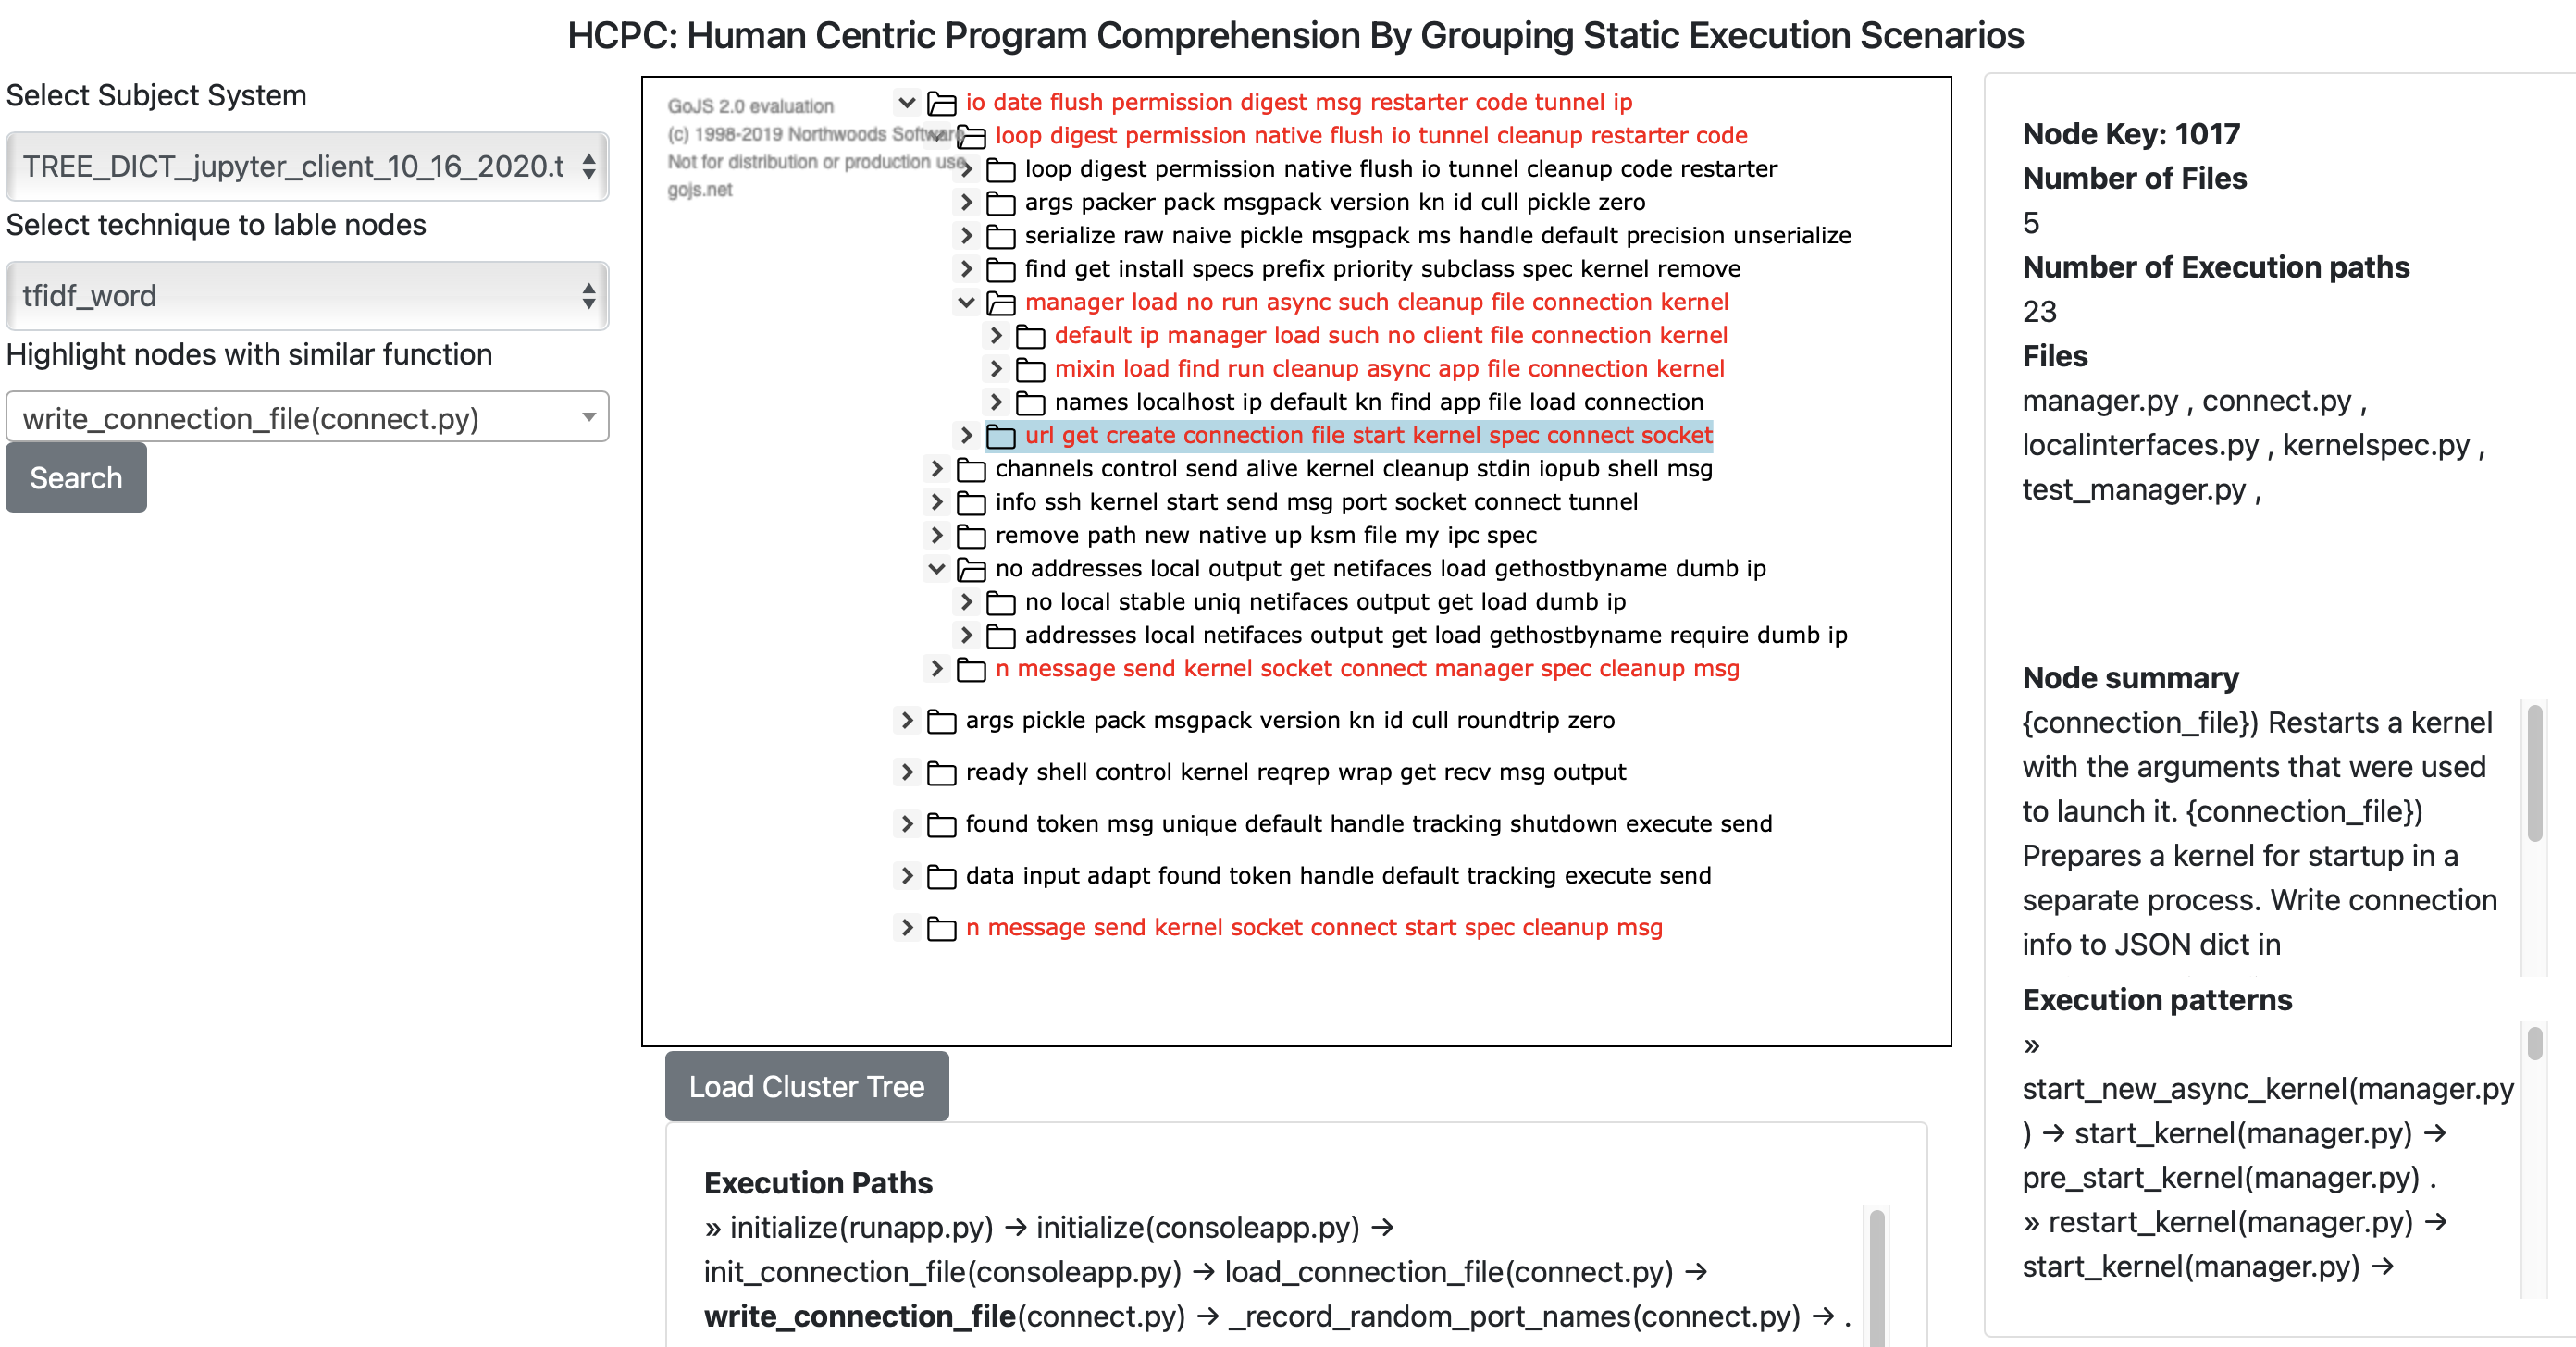
\includegraphics[width=\columnwidth]{figures/hla3/hla3_write_connection_file.png}
  \caption{HCPC tool when focusing on write\_connection\_file method }~\label{fig:tool_write_connection_file}
\end{figure*}

% Discuss write_connection_file
\begin{itemize}
    \item \emph{Create a zmq Socket and connect it to the kernel. return the IP addresses that point to this machine. Write connection info to JSON dict in self.connection\_file. Restarts a kernel with the arguments that were used to launch it. Restarts a kernel with the arguments that were used to launch it. Pass a message to the ZMQ socket to send. Cleanup connection file *if we wrote it*. Given a message or header, return the header. Forgets randomly assigned port numbers and cleans up the connection file. Sends a signal to the process group of the kernel }
    
    From this node summary, we comprehend that in \emph{jupyter\_client} some concepts related to write in connection files are write connection info as JSON dict, cleanup of connection file and forgetting randomly assigned port numbers.
    
    \item \emph{ Restarts a kernel with the arguments that were used to launch it. Prepares a kernel for startup in a separate process. Write connection info to JSON dict in self.connection\_file. replace templated args (e.g. Verify realpath is used when formatting connection file. Walks env entries in templated\_env and applies possible substitutions from current env.}
    
    From this node summary, we comprehend that in \emph{jupyter\_client} some concepts related to write in connection files are restart kernel, creating environments and prepare a kernel startup in separate process.
    
    \item \emph{Load connection info from JSON dict in self.connection\_file. return ip for localhost (almost always 127.0.0.1) set up ssh tunnels, if needed.} 
    
    From this node summary, we comprehend that in \emph{jupyter\_client} some concepts related to write in connection files are set up ssh tunnel, loading connection info from file.
    
    
\end{itemize}

From above discussion with regard to write\_connection\_file method, we can see that HCPC helps to understand relevant concepts for a specific task. 

\section{Human-subject Study}
\label{hla3:human_study}
To evaluate the effectiveness of HCPC, we contacted with \emph{Scidatamanager} development team. We have collected their source code to analyze using our system. We have conducted the study with three developers of the \emph{Scidatamanager} project to find out their opinion about the HCPC tool.

\subsection{Research Questions}
\label{hla3:evaluation}
We want to evaluate the effectiveness of HCPC for helping developers comprehend a software project. We address two research questions:
\begin{itemize}
    \item \textbf{RQ1:} To what extent developers do agree with our approach for getting overview of a project?
    \item \textbf{RQ2:} How helpful is our approach to understand relevant high-level concepts targeting a low-level source code (method)?
\end{itemize}
\subsection{Study Design}
The interview with developers are conducted remotely via Skype. The interview process was divided into four steps:
\begin{itemize}
    \item \emph{Introduction:} First, we brief each participants about our research. Then, we share our screen to show how to use the HCPC tool. We demonstrate the HCPC tool by exploring \emph{jupyter-client} project. We also discuss different components' role to help program comprehension. Later, we asked the participants to go to a specific URL where our application is hosted and share their screen. We informed participants about two parts of the study.  
    
    \item \emph{Feedback on getting overview (RQ1):} In this phase, we asked the participants to explore the ACS tree alongside different components like node summary, execution patterns. We requested them to check whether they can get an  overview of the \emph{SciDataManager} project. We encouraged the participants to express their thoughts while they explore different parts of the system. At the same time, we observed the participants' interaction with the system and noted feedback provided by them. When they explored the tree, we asked them whether the keywords and groups provide any reasonable clue about what the system does. Similarly, we asked them about their opinion on node summary and execution Patterns. We also inquired whether they have any suggestions or expectations for the components to be more helpful.
    
    
    \item \emph{Effectiveness of finding help for specific task (RQ2):} After we complete the second step, we move on to the third phase. In this step, we ask the participants to use the search option to find relevant nodes in the ACS tree and see whether they can find any help to do tasks they recently did. We have encouraged them to remember any recent feature or issue they solved and try to see whether the HCPC tool could help them for completing the tasks. We asked the participants about how helpful Node summary, Execution patterns and the highlight of execution paths can be for someone new to the codebase to accomplish the tasks.
    \item \emph{Open discussion and closing:} At the end, we asked some open-ended questions like suggestion for new features, feedback for existing features. The meetings lasted between 40 to 60 minutes. We ended the meeting thanking the participants for their valuable feedback and time.

\end{itemize}
\subsection{Participants and Subject System Selection}
While observing the HCPC tool output for \emph{jupyter-client} project, we can relate the different nodes content to the components in \emph{jupyter-client} documentation. We decided to conduct the study on a subject system where the team members can participate in the study to evaluate HCPC tool performance on their known codebase. We contacted the \emph{SciDataManager} team whether they could share their source code and participate in the study to evaluate the HCPC. The development team agreed to share the codebase and three of them participated in the study. 
\subsection{Results}
\textbf{Answering RQ1.} Participants agreed that the HCPC tool can help in getting an overview of their project. When we asked the participants, they started to explore the abstraction tree by carefully observing the keywords for each node and expanding to child nodes. The participants agreed that high-level nodes provide hints to the features in their project. For example, participant P3 said, \emph{``I can relate to different basic components from high level nodes. If someone new joins the team, they can start from top nodes and see the path patterns for getting most frequent behaviour and then explore the code-base easily."} Participants appreciated the node summary as it states in plain text what are the purposes of the keywords in the project. Participants also find that when they see node summary for deeper nodes, the summary becomes more precise for specific features. 
According to participant P1, \emph{`` This part is helpful as it states in natural texts instead of a few words. Another interesting fact about the summary is when going deeper the summary became more precise.''} While exploring the execution patterns, we observed that participants find it helpful to know some frequent call sequences in specific nodes. However, participant P2, P3 suggested that having the frequency with the patterns would be interesting to know for understanding the importance. 

In summary, \textbf{Participants find the HCPC tool helpful for getting an overview of their software system with node title, summary and execution patterns.} According to their final feedback for comprehending overview, they pointed out that the HCPC tool has the potential to decrease the getting started time for a project. According to participant P1, they believe  it can help to decrease getting started time around 50\%-60\%.

\textbf{Answering RQ2.} Participants find it useful to be able to search for specific keywords. From the interview, we observed that developers tried to highlight nodes for some recent work they have done or something they are familiar with to check how the HCPC tool is representing the relevant concepts. For example, participant P3 tried to highlight the nodes related to dataset publishing as it is one of the core feature of the project. While browsing the highlighted nodes and its supporting contents (node summary, execution patterns, execution paths), participant P3 identified that it is possible to know similar paths where the function is called. Another interesting observation by participant P2 is, \emph{`` I see the nodes can be searched by functions. In addition, I would love to see filters such as class, files.''} Participant P3 shared from their previous experience that sometimes they have to fix some issues of another project which are not very well documented and they struggle a lot to figure out the abstraction patterns followed in the codebase. Both participants P3, P1 suggested using the search option to explore execution paths will be helpful to decrease time required for completing tasks in those scenarios. Another interesting observation from the interview is for some searches multiple nodes are highlighted which shows the specific functions being used in different scenarios. We observe participants were enthusiastic to know what are the different directions the function is being used by going deeper in the abstraction tree. In addition, participant P1 shared that many times they try to search the codebase with some keywords using the find option provided by the editor to retrieve relevant files. However, the search result does not show any order or how these classes or methods are being called. They suggested that with the execution patterns and paths  the HCPC tool can help to convert the raw find workflow into more execution based search process. In summary, \textbf{the feedback from the participants and our observation during the interview indicate that it is viable that the search option of the HCPC tool has the potential to help in day-to-day software maintenance activities. } 

% To Do using find button for searching which do not have any order

During our open-ended questions and suggestions, we found valuable feedback for future development and adaptation of the HCPC tool. One important suggestion is to incorporate automatic comment generation techniques for methods which have no comments. This will be a valuable future work suggestion for our HCPC tool, as it will be helpful for projects which do not follow best practices. Another worth mentioning future work suggested by participant P2 is to generate a report of the abstraction structure where developers can edit the components' names according to their understanding from the HCPC tool. This report can be used as a documentation of the project structure from a static execution perspective. In addition, participants suggested to enable the option to export projects from GitHub which will be useful for quickly exploring a new codebase. From the above discussion, \textbf{we can conclude that the HCPC tool can help to get an overview of a software project from a static execution perspective and can be used to help doing a specific task in hand.}


% TODO
% github, report generation 


\subsection{Threats to Validity}
To address external validity, we have collected a software project which is developed in industry settings instead of working with a sample project. We have selected a professionally developed project to ensure generalizability to some extent. Although the subject system is written in Python, our approach will work with both static and dynamic typed language as our approach depends on only caller-callee relationship between methods. 

To address internal validity, we have tried to minimize any communication issue by repeating the feedback when in doubt. We acknowledge that our sample size for participants in the study is small. However, our participants' are experienced in the subject system and we got repetitive feedback which indicates acceptance to some extent. We asked open-ended questions at the end so that participants are able to provide feedback outside the questions asked. 




\section{Conclusion}
In this study, we have proposed two new approaches to enhance the abstract code summary tree for program comprehension. First, we change the similarity metrics for comparing execution paths. In previous studies, Jaccard distance is used which only considers the content not the sequence. Therefore, in this study, we have changed the similarity metrics to strike\_a\_match algorithm. Second, we changed the clustering approach for more precise grouping of the execution paths. Previous studies suggested to use the hierarchy tree for browsing. However, from previous studies we found that hierarchy tree has abundant abstraction nodes which hinders going deeper levels.
We used cluster flattening technique which reduces redundant abstraction nodes from hierarchy tree. We have built an interactive system to explore the new abstraction tree with supporting information alongside searching the tree. To evaluate, the system we have conducted a human subject study. We find that our system can be useful for getting acquainted with a software project as well as accomplishing tasks in hand.  
